\documentclass{article}
\usepackage[utf8]{inputenc}
\usepackage{amsfonts,amsmath, amsthm}
\usepackage{geometry}
\usepackage{url}
\usepackage{appendix}
\usepackage{hyperref}
\usepackage{caption}
\usepackage{subcaption}
\usepackage{graphicx}
\usepackage[dvipsnames]{xcolor}
\geometry{margin = 1.25in}
\title{Collaborative Replication of Applicable Mean Field Disease Modeling Studies}
\author{}
\date{}

\usepackage{natbib}
\usepackage{graphicx}

\begin{document}

\maketitle

\section{Introduction}
Mathematical disease models have been extensively used for estimation, prediction, forecasting and public health policy guiding. The latest example being for CoVid-19 pandemic, and in the past for Zika disease international public health emergency, etc. \cite{paixao2016history}

\paragraph{Motivation.} As has been done for biological and psychological sciences research previously [cite], replication studies have proven to be an important resource for validity and review of methodologies in the respective fields. If done collaboratively, the knowledge and reliability of the produced research in the field increases \cite{nosek2020best}.

\paragraph{Goals and Objectives.}
While attempting to reproduce results from an arbitrary selection of disease modeling peer-reviewed publication, we aim to assess and analyze the following

\begin{enumerate}
    \item Whether the results in the paper are reproducible. If not, what would have made it reproducible.
    \item Whether the assumptions behind the choice of the model are justified for the research question and are reported.
    \item Whether the assumptions behind the choice and implementation of different parameter values are reported.
    \item What was the target audience (based on the journal it was published in) and whether the terminologies used in the model description suitable for it.
    \item Sensitivity of the model outcomes to the parameters whose reported value was an arbitrary assumption.
    \item Whether the data and code made publicly available.
\end{enumerate}

Commonly noticed factors that made any results reproducible from the selected papers are
\begin{enumerate}
    \item not reporting initial conditions,
    \item parameter estimates used for results not consistent throughout the paper, 
    \item assumptions behind the choice of the parameter definition and estimates not always reported.
\end{enumerate}

\paragraph{Hypotheses.}
We hypothesize the following factors to be responsible for these issues
\begin{enumerate}
    \item Compartmental models originated a long time ago and hence the first principle mechanistic assumptions behind them are lost and forgotten due to the overwhelming number of the models designed and used.
    \item Pressure for fast publications lead to authors not being able to report details.
    \item The errors slipping through the review process may indicate a lack of a transdisciplinary review committee.
    \item Discrepancy between the backgrounds of the authors and readers reflecting on the need for more centralized modeling practices with interdisciplinary collaborations \cite{kretzschmar2020disease}.
\end{enumerate}

\paragraph{Method and Approach.} We invite the authors of the papers included in this replication study to bridge the communication gap. With their assistance we will exactly identify the pieces of information needed for successful reproduction of the reported results. They are encouraged to volunteer their other papers to be included in this study. Through this meta-analysis, we collaboratively reflect on the potential changes to the scientific process to maximize reproducibility.


\paragraph{Expected Outcome.} We collectively come up with 
\begin{enumerate}
    \item a checklist for assumptions for using SIR type models for the intended application
    \item a protocol for reporting the methods
\end{enumerate}
Additionally, we intend to connect the independent research labs working on a similar problem, motivate interdisciplinary collaborations and encourage making the resources to reproduce publicly available.

\section{Initial Questions and Tasks}
\begin{enumerate}
    \item Do we include only the corresponding author of the selected papers or all of them? \textcolor{ForestGreen}{All or whoever responds?}
    \item How to be disarming when proposing and contacting the authors? \textcolor{ForestGreen}{Pointing at Figure \ref{fig:nature_replication}}
    \item What should be the extent of the authors' involvement? \textcolor{ForestGreen}{Permission to use their paper without burning bridges, volunteer their other paper(s) for analysis}
    \item Draft the contact email.
    \item Include more papers from more popular journals.
\end{enumerate}

\begin{figure}
    \centering
    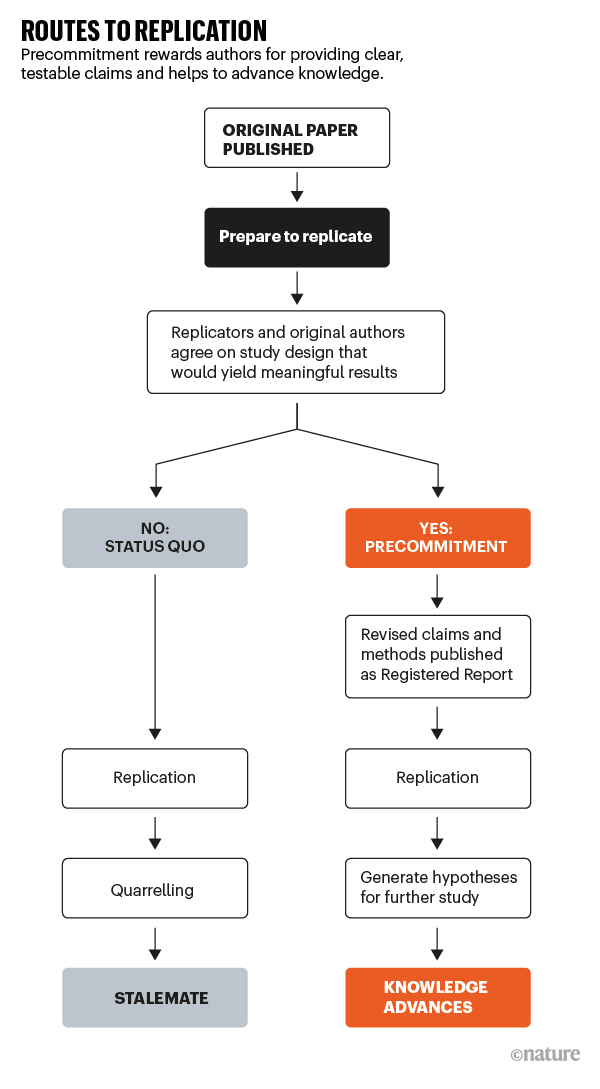
\includegraphics[scale = 0.4]{replication.png}
    \caption{Source: \cite{nosek2020best}}
    \label{fig:nature_replication}
\end{figure}
\bibliographystyle{plain}
\bibliography{paper2.bib}

\end{document}